\documentclass{tufte-handout}

\title{On ultimate; O2: secondary middle, left centre or popper}
\author[James Reynolds]{James Reynolds}

%\date{28 March 2010} % without \date command, current date is supplied

%\geometry{showframe} % display margins for debugging page layout

\usepackage{graphicx} % allow embedded images
  \setkeys{Gin}{width=\linewidth,totalheight=\textheight,keepaspectratio}
  \graphicspath{{graphics/}} % set of paths to search for images
\usepackage{amsmath}  % extended mathematics
\usepackage{booktabs} % book-quality tables
\usepackage{units}    % non-stacked fractions and better unit spacing
\usepackage{multicol} % multiple column layout facilities
\usepackage{lipsum}   % filler text
\usepackage{fancyvrb} % extended verbatim environments
  \fvset{fontsize=\normalsize}% default font size for fancy-verbatim environments

% Standardize command font styles and environments
\newcommand{\doccmd}[1]{\texttt{\textbackslash#1}}% command name -- adds backslash automatically
\newcommand{\docopt}[1]{\ensuremath{\langle}\textrm{\textit{#1}}\ensuremath{\rangle}}% optional command argument
\newcommand{\docarg}[1]{\textrm{\textit{#1}}}% (required) command argument
\newcommand{\docenv}[1]{\textsf{#1}}% environment name
\newcommand{\docpkg}[1]{\texttt{#1}}% package name
\newcommand{\doccls}[1]{\texttt{#1}}% document class name
\newcommand{\docclsopt}[1]{\texttt{#1}}% document class option name
\newenvironment{docspec}{\begin{quote}\noindent}{\end{quote}}% command specification environment

\begin{document}

\maketitle% this prints the handout title, author, and date



%\printclassoptions
This document is about 
playing secondary 'middle'
(vertical), 
left-central cutter 
(horizontal), 
or popper 
(zone) 
on offence\footnote{
Referred to here 
as position O2.
This
is part of a series, 
available at
\url{https://github.com/James-Reynolds/Ultimate-strategy-and-tactics}}.
Let the handlers 
deal with catching the pull, but
as you run downfield
try to 
see
what defence structure
is being used. 
%\footnote{It could be:
%person-match defence,
%person-match-last-back-helps,
%person-match-with-a-poacher,
%person-match-with-lots-of switching,
%force-middle,
%force-straight-up,
%zone-3-3-1-force-middle-
%zone-3-3-1-force-sideline
%zone-3-3-1-force-forehand
%zone-3-3-1-force-backhand
%zone-3-3-1-etc
%zone-3-2-2, 
%zone-2-3-2, 
%zone-1-3-2-1 (puppy-fence),
%clam,
%or something else}.

\section{Beating person-match defence with a vertical stack}\label{sec:vertical}

\begin{marginfigure}%
  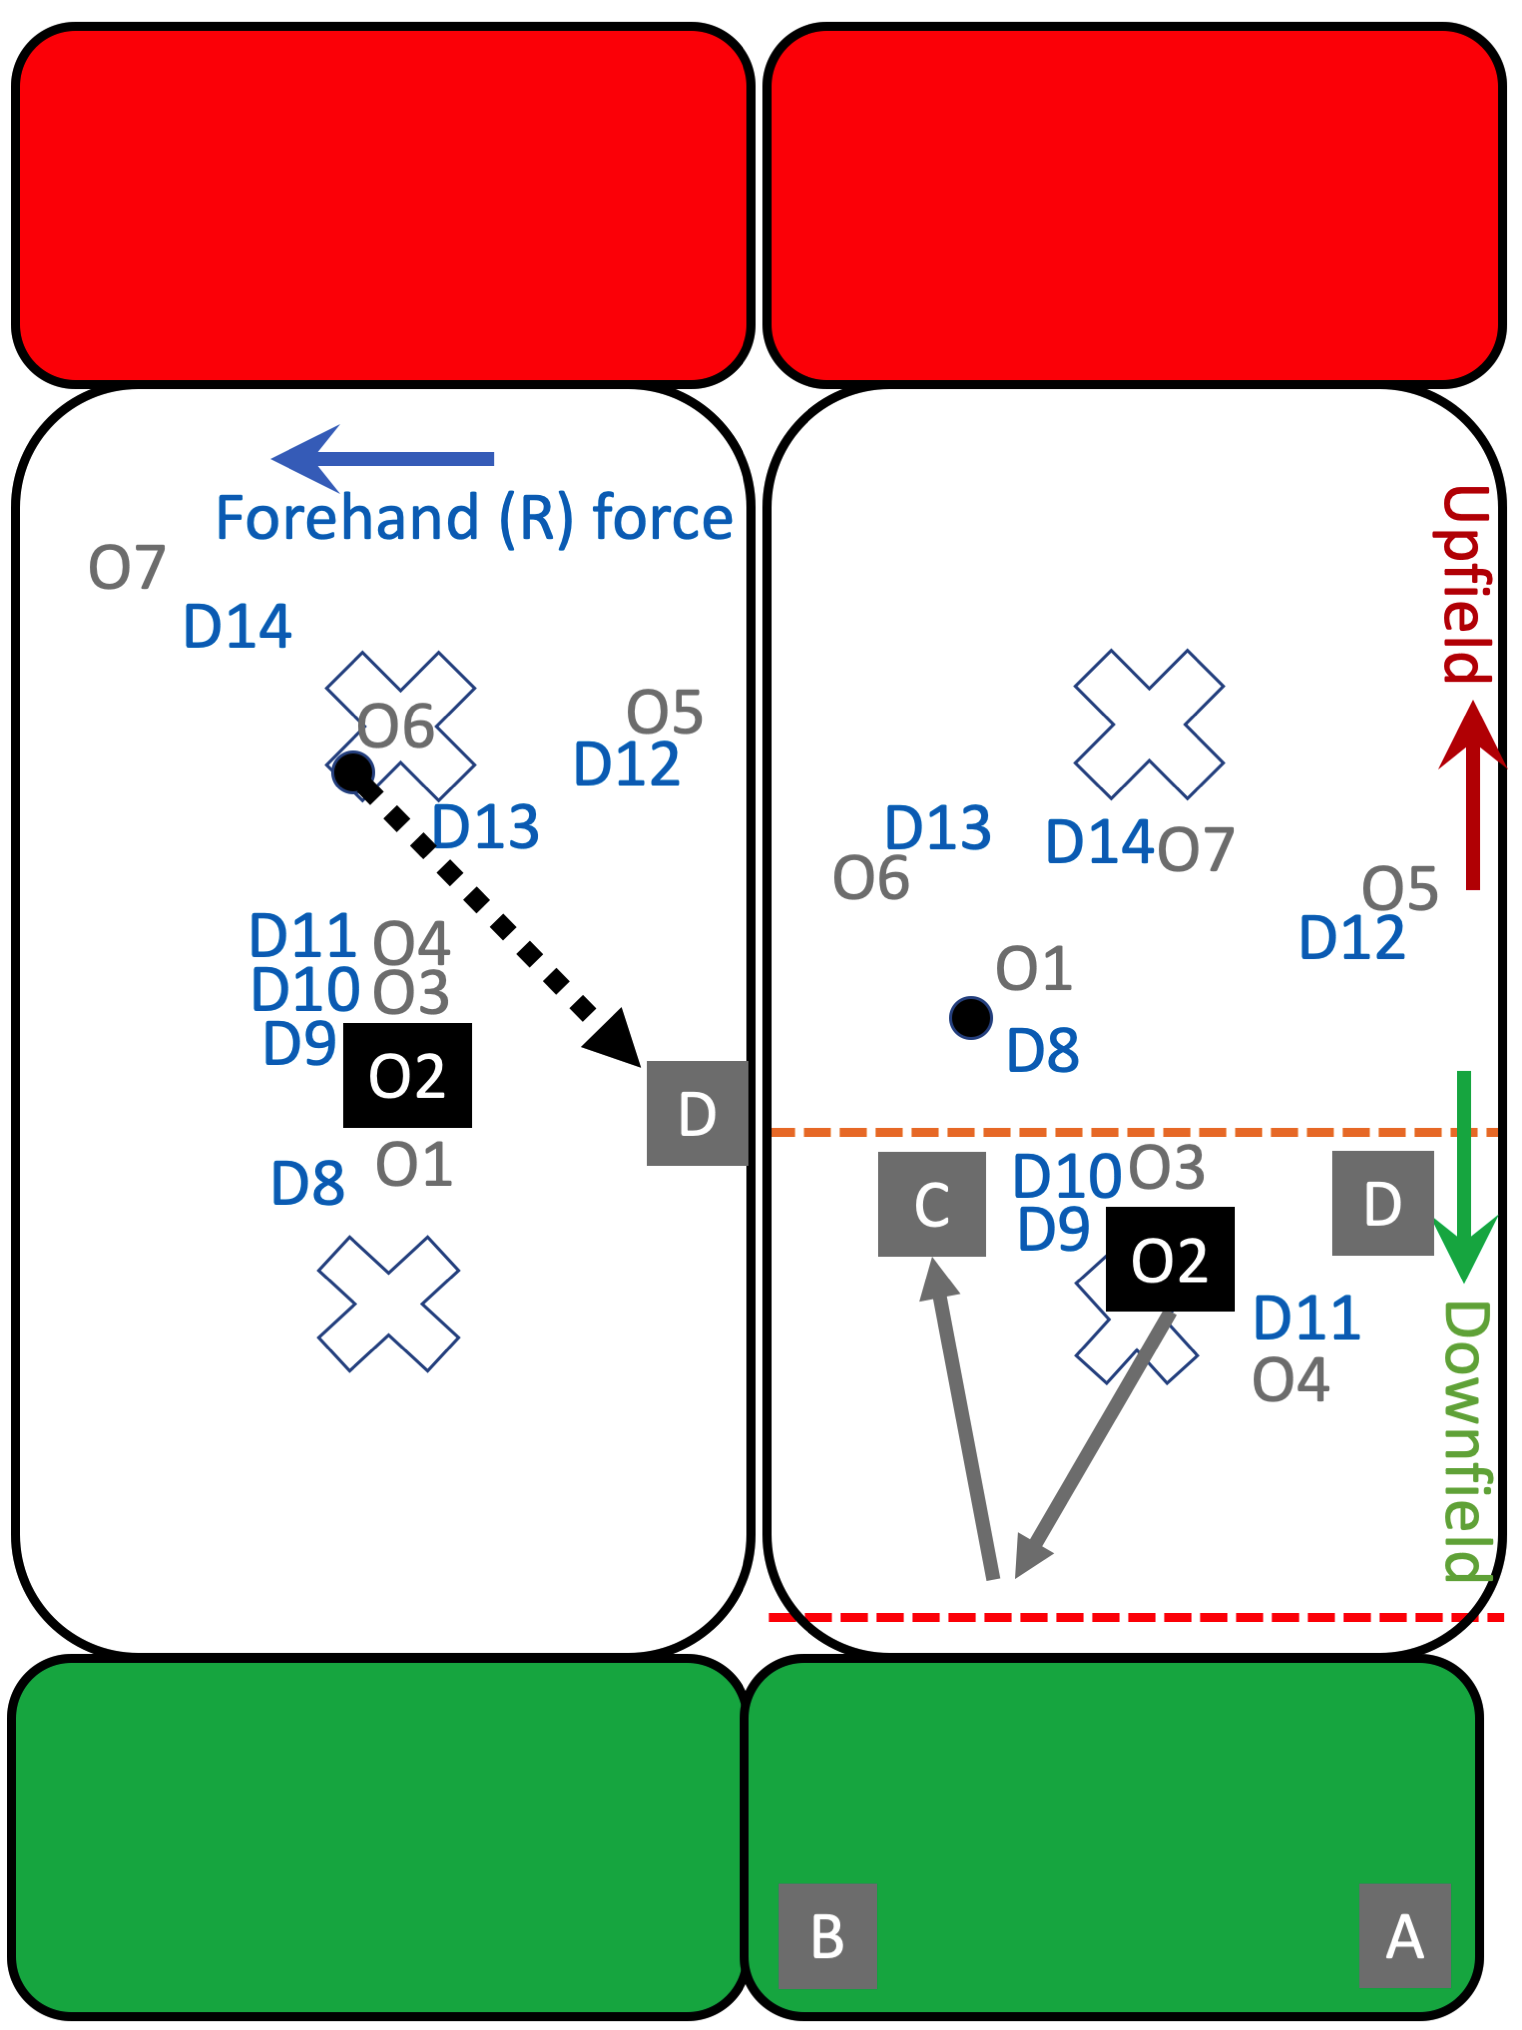
\includegraphics[width=\linewidth]{O2-vertical}
  \caption{Vertical stack: 
  starting position (left),
  and development (right)}
  \label{fig:O2-vertical}
\end{marginfigure}


Figure \ref{fig:O2-vertical} (left) shows 
a situation 
with: 
a brick called;
a forehand force; 
person-match defence; 
and your team using 
a vertical stack formation.
As secondary middle, 
(O2) 
your role 
will likely 
involve cutting 
\smallcaps{after} 
the primary middle 
(O1)\footnote{
Especially as being 
in the middle of the vertical stack,
as shown in 
Figure \ref{fig:O2-vertical} (left)
it is difficult for 
you to make a cut 
without causing 
a pick. 
In contrast, 
Figure \ref{fig:O2-vertical} (right)
shows O1 
having cut upfield 
and received 
a pass 
on the open side, 
which immediately 
frees you 
(O2) 
to cut 
from the back of the stack,
with less chance 
of a pick occuring.}.
However, 
in Figure \ref{fig:O2-vertical} (left)
O6 is shown
potentially throwing 
a break throw to D,
which you 
(O2),
or any of the other cutters
(O1. O3, O4) 
might be able to run onto 
after it is thrown. 
All the defenders 
(D8-D11) 
are on the wrong side, 
so you are all open 
to that space.
However,
you will likely need to 
stay still before it is thrown 
as if you 
cuts towards D 
\smallcaps{prior to the disc being thrown} 
then there is likely 
to be a pick\footnote{
Picks occur
when a  
defender is 
obstructed from 
following someone 
they are marking.  
So maybe stand still
until it's thrown 
so any pick 
might not affect the pass itself
(meaning that it stands), 
and D9 
only gets to catch up 
to put the force on earlier.}.

There are many 
different ways that the 
play might develop.
Figure \ref{fig:O2-vertical} (right) shows 
the disc having been thrown 
to O1
on the back-under 
cut 
to the open side. 
O4 is indicated 
clearing 
or cutting 
deep on 
the break side. 
The stack is shown having 
moved further downfield, 
in response to the pass
to O1
with you, 
having waited
for O1 to cut first,
still in the stack
together with
O3. 
This leaves 
you 
available to make 
cuts
to A-D, 
\smallcaps{now that O1 has the disc.} 


It is this timing 
that is important 
when playing 
in a secondary cutter position. 
O2 is called secondary middle, 
because you cut second, 
not because the position is of secondary importance. 
Ideally,
only  
(maybe) two of the four cutters
(O1-4) 
will be out of the stack (cutting)
at any moment.
Otherwise, 
you will likely 
get in each others way, 
and/or run out of cutters 
in position 
to cut next.  
Staying  
between 
the dashed 
horizontal 
lines 
may also help when cutting\footnote{ 
The position of 
the lines vary
with the position of the disc
and with how far the thrower  
can or will 
throw. 
However, 
if you go 
downfield of the dashed red line 
before the disc is in the air,
D9 may be able 
get to
A or B 
before the disc,
intercepting 
or preventing 
deep throws to 
you or others. 
Similarly, 
if you go 
upfield of the dashed yellow line
then D8 may 
be able to help
prevent dump throws from O6
to O5 
or O7.}.

Vertical works
against other person-match defences. 
But it might need 
some adjustment.
For example
against: (1) RH-backhand-force: mirror the above; 
(2) last-person-covers-the-deepest-threat
you may need to coordinate with O1 
to overload D8 (deep) 
or D9 (under); or
against (3) a straight-up force, 
maybe stay in the stack 
while the handlers move the disc around
until there's an opportunity
for a huck without a marker, 
or if you do cut under go out to the sideline. 


\subsection{Beating person-match defence with feldrunner}
\label{sec:feld}
Figure \ref{fig:O1-horizontal} (left) 
shows a feldrunner formation, 
with 4 handlers, 
2 cutters 
in the endzone,
and you 
(O1) 
left  
isolated 
in the centre
as the focus. 
O6 can throw 
to A,
B, 
C 
or D. 
If D8 looks at you, 
stand still and 
O6 can throw it 
to your advantage. 
If D8
looks at O6, 
cut to A-D. 
Instead, 
O6 might reset 
to O4, O5 or O7, 
for them to 
throw to you. 
With the disc 
you can throw
to cuts from O2-3, 
or dump and repeat. 

\begin{marginfigure}%
  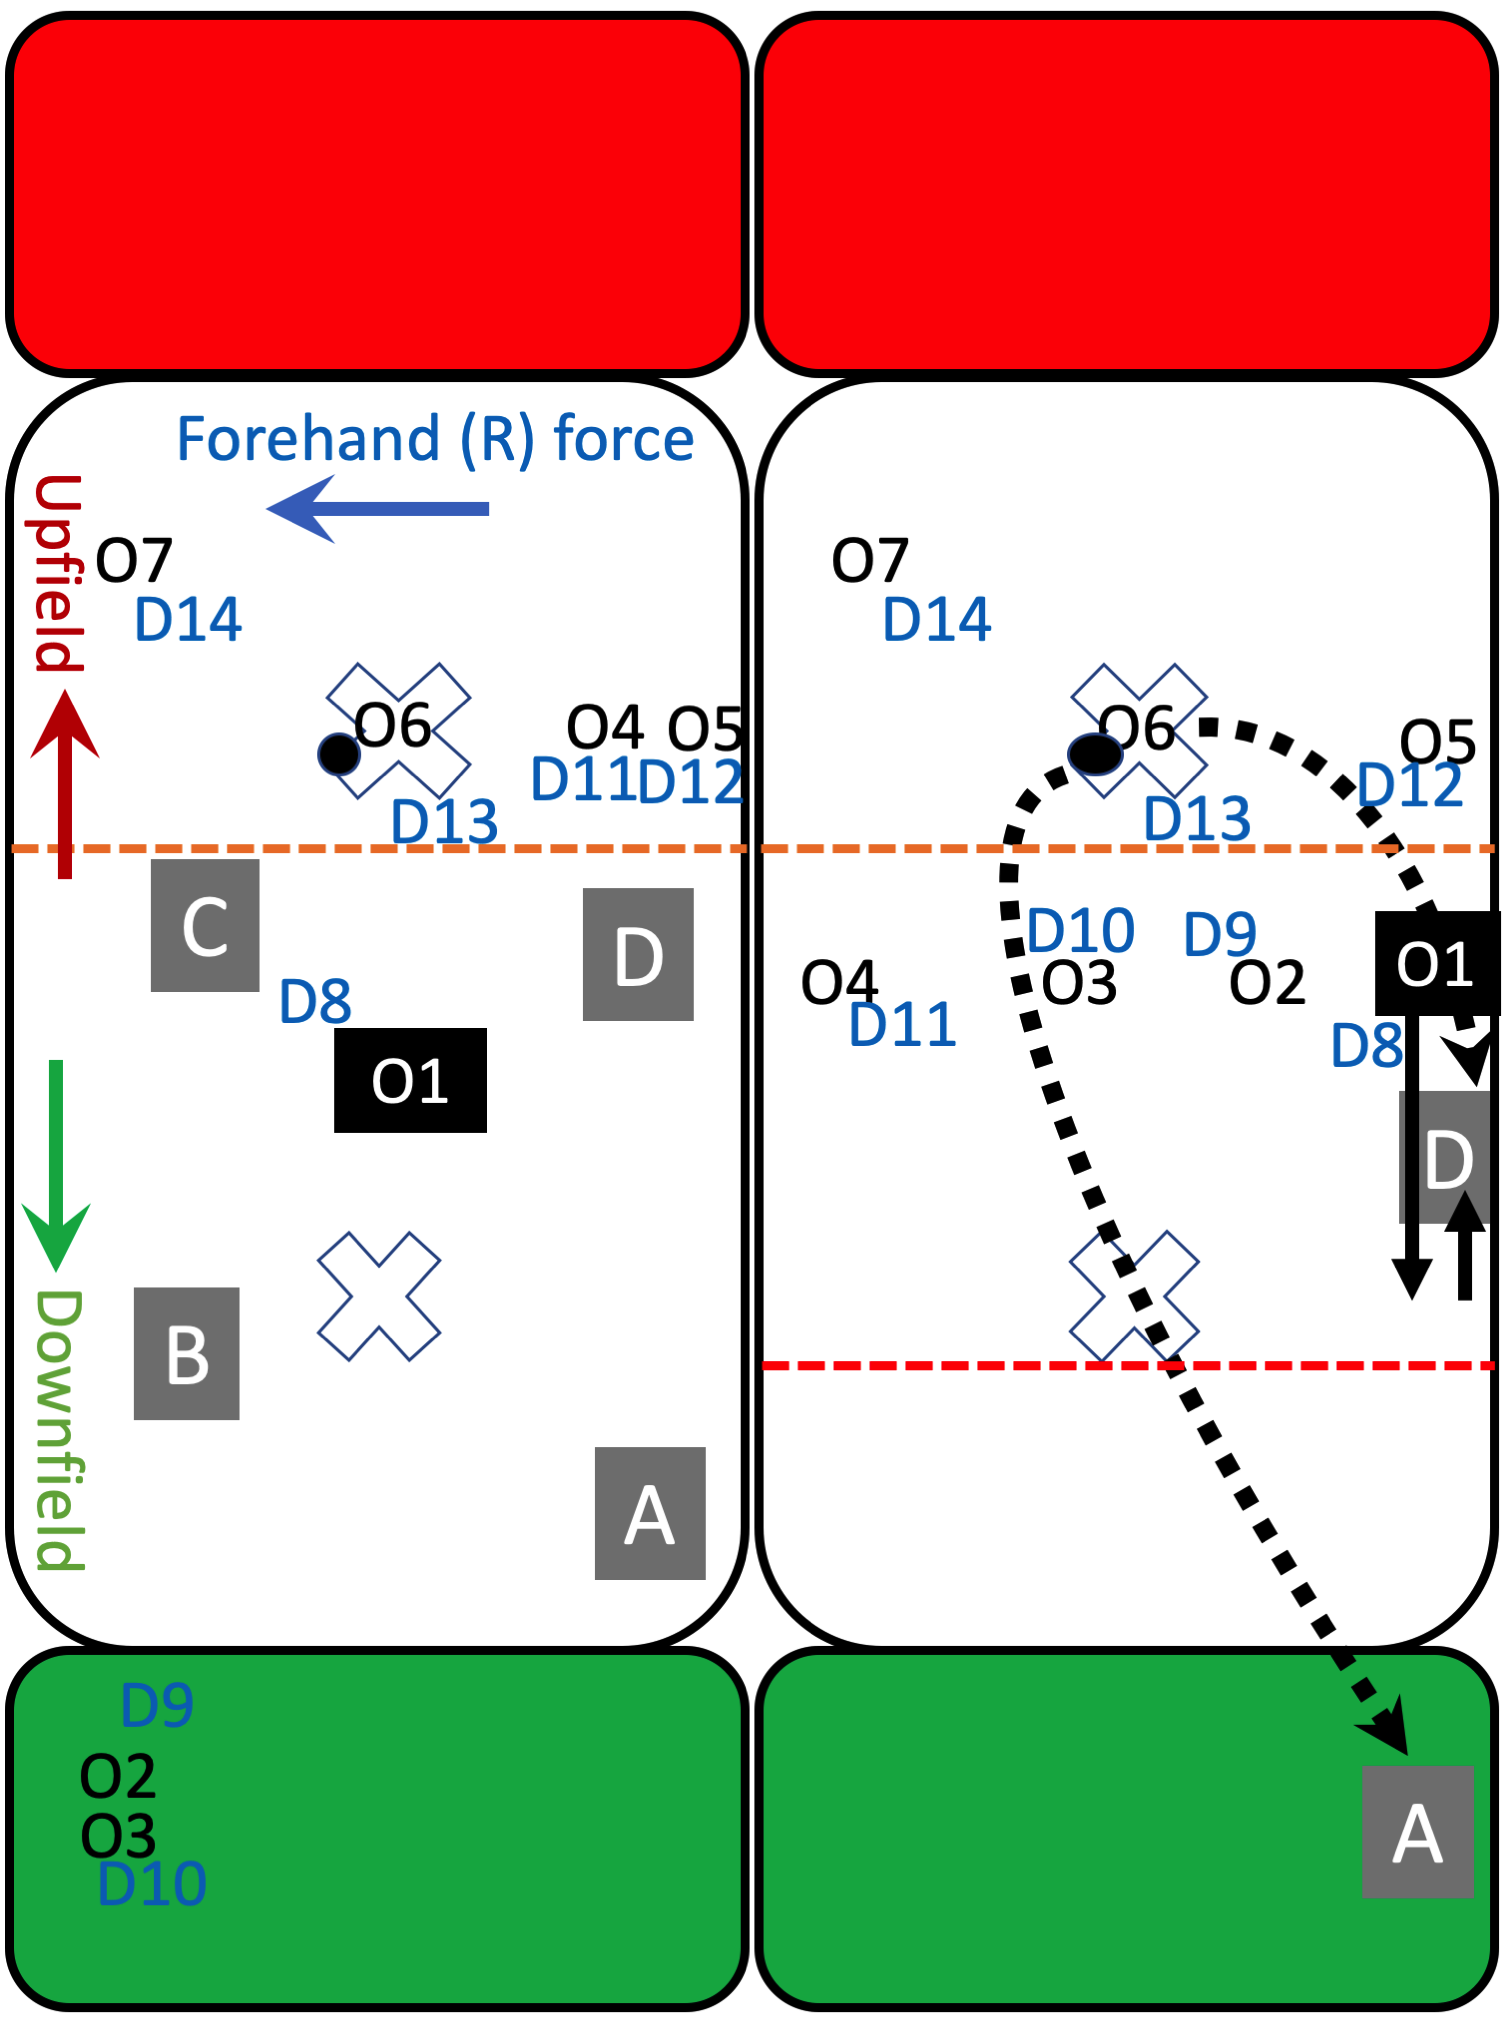
\includegraphics[width=\linewidth]{O1-horizontal}
  \caption{Feldrunner (left) and horizontal (right)}
  \label{fig:O1-horizontal}
\end{marginfigure}


\subsection{Beating person-match defence with a horizontal stack}\label{sec:horizontall}
Basic horizontal stack 
involves cutting
upfield and downfield (black arrows)
within your quarter of the field\footnote{
Other cuts
can work, 
but might need
communication,
e.g. diamond cuts 
involve you trading places 
with O2.}. 
Figure \ref{fig:O1-horizontal} (right) shows 
O1 on the left wing. 
O6 
can potentially 
throw to you 
at A 
or D\footnote{
Black arrows
show how a back-under cut 
opens space 
for this throw.}. 
However, 
O6 throwing to 
O2, O3 or O4  
may be easier. 
Hence,  
you may wish to 
wait and 
cut later. 
If you do get the disc 
at D 
a huck to 
A for O2 or 
to B for O4 
may be effective.
Otherwise, 
get it to the middle of the field 
with a dump to O5 or O6. 

A typical pattern
is that D8 (marking you)
will try to help 
D9, D10 and D11 
by poaching deep.
To beat this 
you can: 
trade spots with O5;
move to the open side, 
between D10 and O6; or 
stay still 
on the left wing,
so O6 can 
get it to you 
quickly
with a hammer 
or blade.

\section{Beating zone defence}\label{sec:zone}

\begin{marginfigure}%
  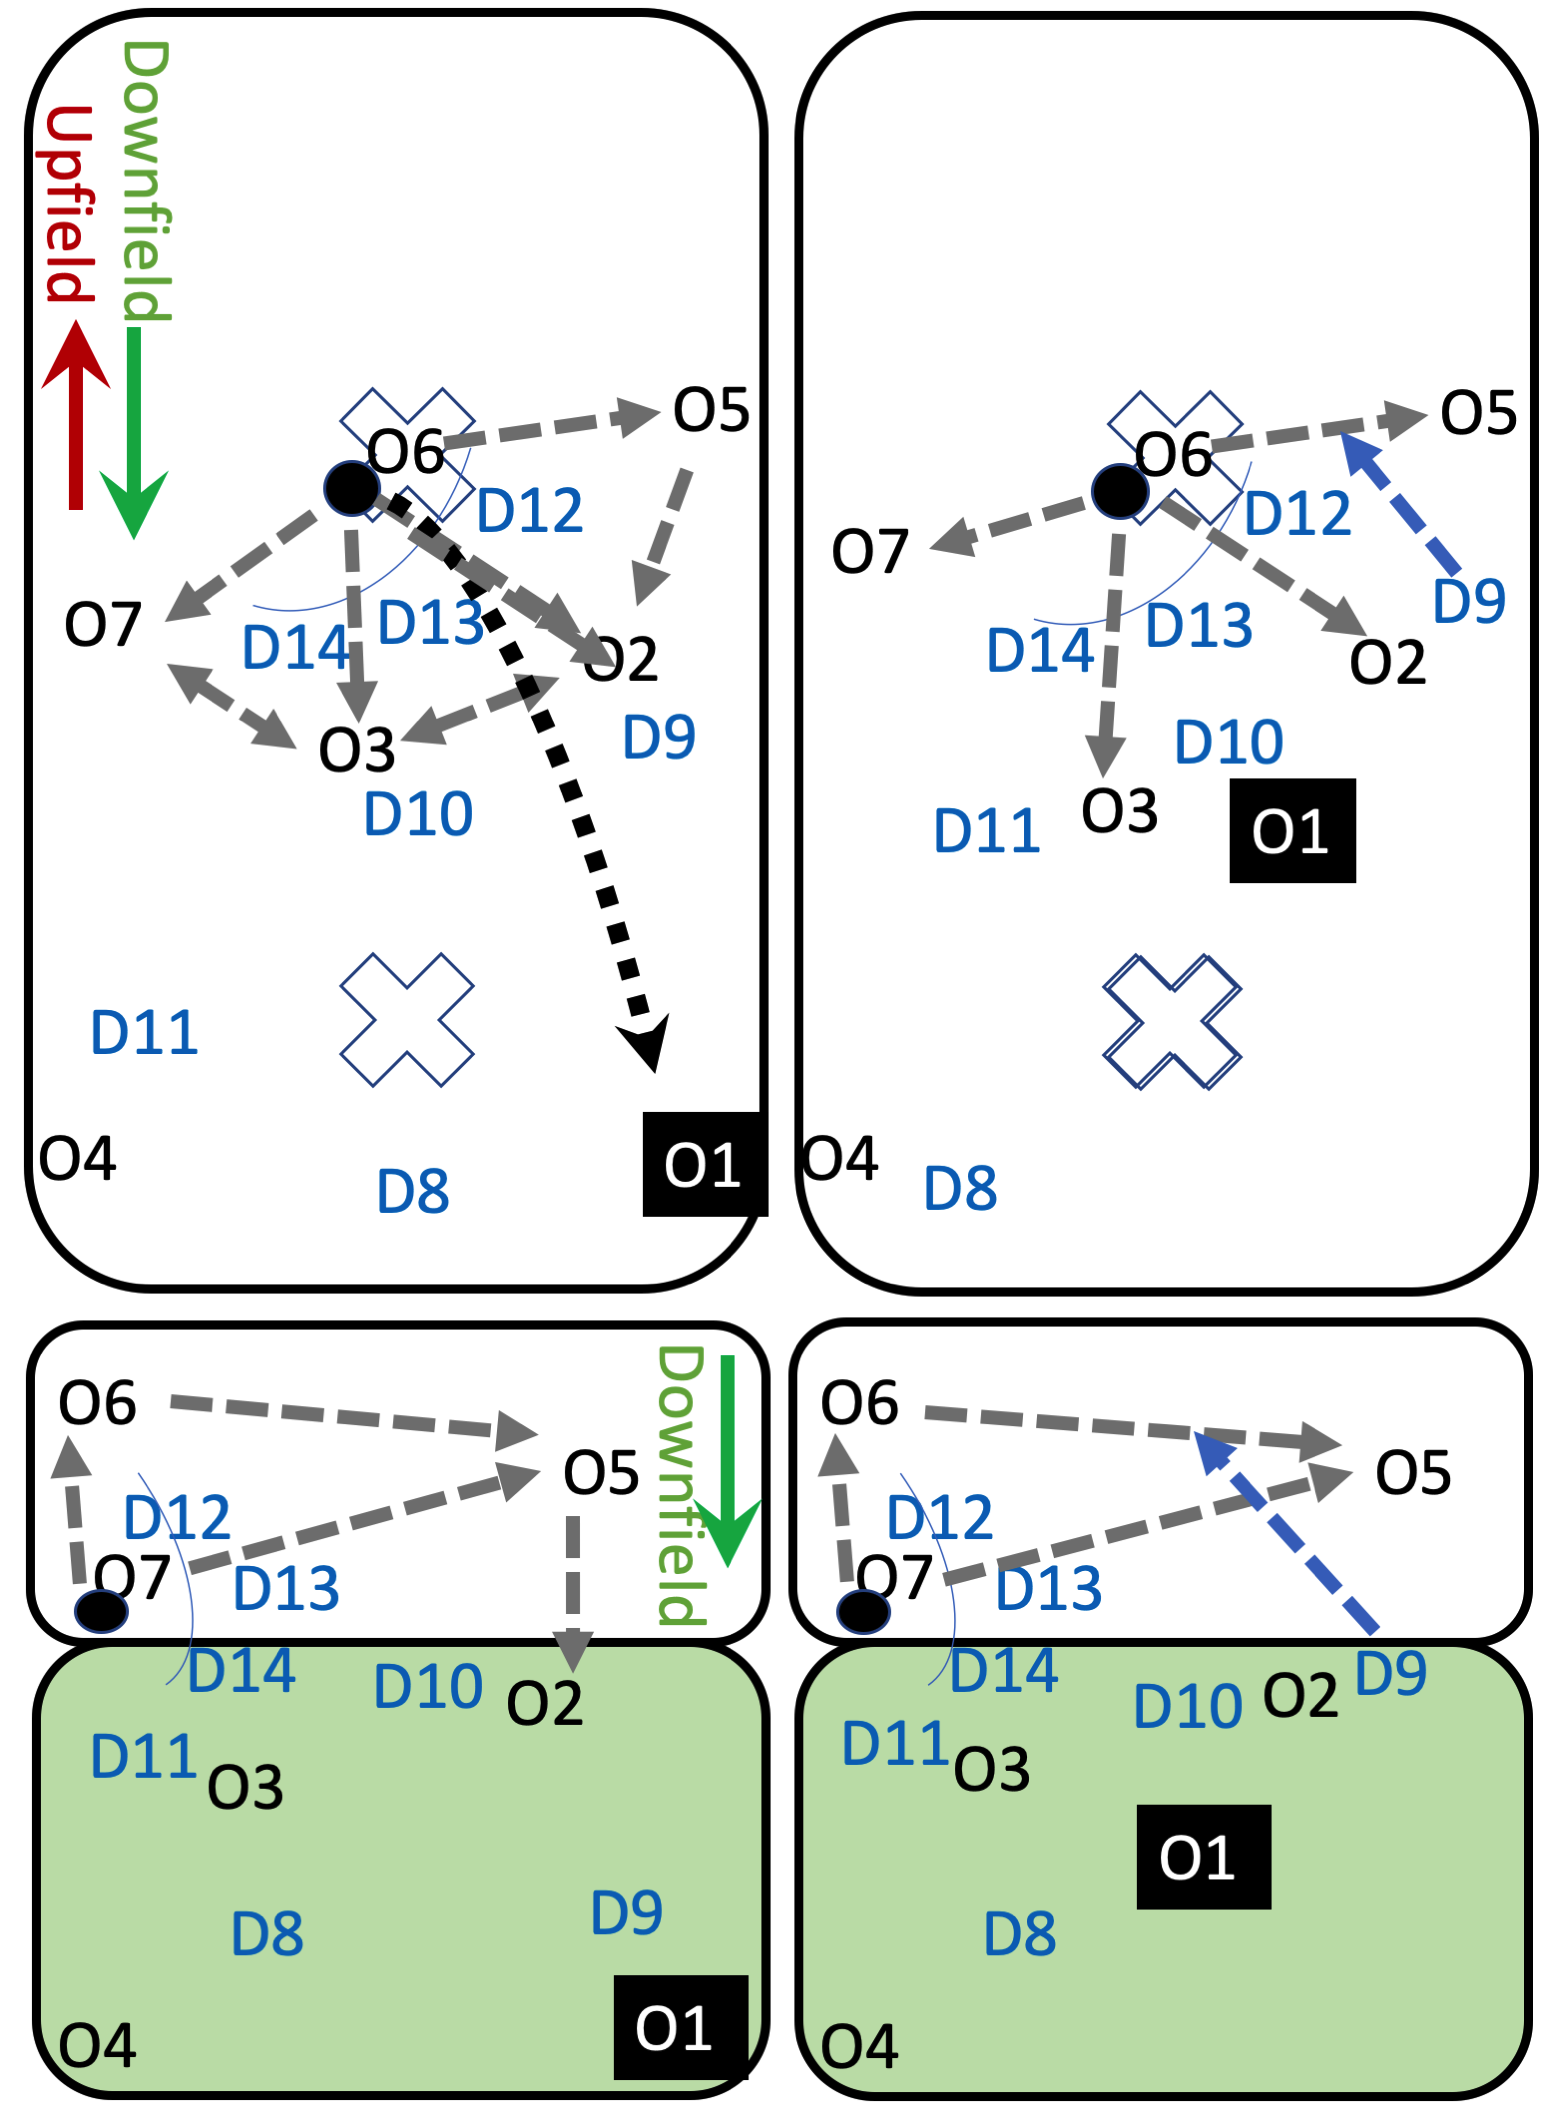
\includegraphics[width=\linewidth]{O1-zone331}
  \caption{effective formations against 331 zone: 
  general (top left)
  and close to the endzone (bottom left); and 
  less effective formations (top, bottom right)}
  \label{fig:O1-zone331}
\end{marginfigure}

Vertical stack 
probably won't work. 
Instead, your 
team needs to 
spread out. 
Three ways to beat a zone are:
(1) over;
(2) round; or
(3) through. 
Figure \ref{fig:O1-zone331}
(top left)
shows this 
against a 
3-3-1 zone. 
Figure \ref{fig:O1-zone331} (top left)
shows a throw 
direct 
from O6 
over to you\footnote{
This may be a 
blade or
hammer, 
to get it 
to you
as quickly as possible.
So it may help to 
stand still 
and look at O6.}.
Otherwise, 
O6 might throw
over or through (to O2 or O3), 
or round (to O5 or O7)\footnote{
You, 
O2, 
O3 and
O5
might then split
D9-10
to make ground 
before the cup 
(D12-14) catch up. 
Once they do, 
dump to O6 
so all 7 of your players
are involved again.}. 

If the defence 
continues to play zone 
once the disc 
gets close to the endzone, 
you (O1) 
and the other wing (O4) 
can \smallcaps{go and stand 
on the back corners}
(Figure \ref{fig:O1-zone331} (bottom left)\footnote{ 
The defence 
will either  
leave you open,
or cover you
at the corner
(D8 
or D9), 
making more space 
for O2, 
O3 and
O5-7 
at the front of the endzone.}.
Figure \ref{fig:O1-zone331} (bottom right) shows 
how the further 
you are from the back corner 
the more D8/9 
can cover both you
AND others,, 
and the harder 
it is to throw direct to you.
D9 might even be able to get a block
on a throw to O5
(dashed blue line). 
This applies also when 
not close to the endzone 
(top right),
If you crowd O2 and O3,
D8 only has to cover O4, 
and D9-11 get to cover 
you (O1),
O2, 
O3 and 
O5.

\section{Beating clam defence}\label{sec:zone}
Clam mixes person-match 
and zone defence styles\footnote{
Involves defenders 
switching 
so as to cover 
an area. 
For example, 
in Figure \ref{fig:O1-vertical}(left) 
D8 
(the deep-deep) 
might cover 
O1 deep, 
but then switch with D11 
(open-side wing)
to cover O4's cut deep, 
while D11 covers 
the O1 
cut to C.}.
Whereever you cut, 
one or more defenders
will likely have you
(at least somewhat) covered. 
As O1, 
you might
coordinate 
with O2
to overload
D8 or D9.



\end{document}
